\subsection{Problema del MCS entre cografos y grafos completos}

En esta sección se presenta un algoritmo exacto para resolver el problema en cuestión para el caso particular en que los dos grafos de entrada son un cografo y un grafo completo, respectivamente. El problema del MCS para este tipo de grafos de entrada puede resolverse en tiempo polinomial, debido a características particulares de este tipo de grafos.

En principio, si consideramos el problema del MCS entre un grafo cualquiera G y un grafo completo Kn, se deduce fácilmente que si $|Kn| \geq |G| \Rightarrow MCS(G, Kn)$ = $G$. Por lo tanto, el caso interesante que se busca resolver es cuando $|G|$ > $|Kn|$.

Para esto, el algoritmo presentado aprovecha la siguiente definición recursiva de un cografo:

\emph{def. \textbf{Cografo}
\begin{enumerate}
\item El grafo trivial es un cografo.
\item La unión ( $\cupdot$ ) disjunta de dos cografos es un cografo.
\item El join ( $\lor$ ) de dos cografos es un cografo, donde $G1 \lor G2 = \overline{\overline{G1} \cupdot \overline{G2}}$.
\end{enumerate}
}

\subsection{Explicación detallada del algoritmo}

El algoritmo propuesto utiliza la técnica de programación dinámica. Aprovechando la definición recursiva de los cografos, dividimos el problema en subproblemas más chicos. Dada la definición, un cografo puede ser un grafo trivial, unión o join de dos cografos. 
Se define la siguiente función recursiva:

$f(G, K, i) = MCS(G, K)$ usando $i$ nodos, con $i \leq min \{|G|, |K|\}$

donde:

\[ f(G, K, i) = \begin{cases} \label{formulacionRecursiva}
      G & si\ G\ trivial \\
      \underset{0 \leq j \leq i}{maxAristas}\ \{ MCS(G1, K, j) \cupdot MCS(G2, K, i-j)\}
      & si\ G = G1 \cupdot G2 \\
      \underset{0 \leq j \leq i}{maxAristas}\ \{ MCS(G1, K, j) \lor MCS(G2, K, i-j)\}
      & si\ G = G1 \lor G2
   \end{cases}
\]

La solución que buscamos, entonces, es: $f(G, K, min \{|G|, |K|\})$.

\subsubsection{Correctitud de la formulación recursiva}

\begin{itemize}
\item \textbf{Caso trivial.} El MCS de un grafo trivial con un grafo completo es ($\{v\}$, $\{\}$), donde $v$ es el único nodo de $G$.
\item \textbf{Caso $G$ es unión de cografos $G1, G2$.} Por transitividad, MCS($Gi, K, j$) $\in G$ pues es subgrafo de $Gi$ y $Gi$ es subgrafo de $G$ $\forall i \in (1,2)$. Además, toda arista y nodo del $MCS(G,K,j)$ de $j$ vertices pertenece bien a $G1$ o a $G2$. Por lo que podemos calcularlo quedándonos con el MCS de máxima cantidad de aristas resultante entre todas las combinaciones posibles de usar $x$ cantidad de nodos de $G1$ y $j-x$ nodos de $G2$ ($x \in [0..j]$). Para ver cuál es el mejor MCS resultante es necesario calcular el x que maximice la cantidad de aristas de la unión entre los $MCS(G1,K,x)$  y $MCS(G2,K,j-x)$ (para todo $x$ válido), ya que vale el principio de optimalidad. Si utilizáramos otro subgrafo de $G1$ o $G2$ que no fuera MCS del mismo, entonces el MCS resultante para $G$ no sería óptimo, pues podríamos intercambiarlo por el óptimo y obtener un MCS mejor para $G$.
\item \textbf{Caso $G$ es join de cografos $G1, G2$.} Para este caso, debemos considerar las aristas que se agregan al hacer el join. Al igual que en el caso anterior, todo nodo del $MCS(G,K,j)$ de $j$ vertices pertenece bien a $G1$ o a $G2$. Por lo que podemos calcularlo quedándonos con el MCS de máxima cantidad de aristas resultante entre todas las combinaciones posibles de usar $x$ cantidad de nodos de $G1$ y $j-x$ nodos de $G2$ ($x \in [0..j]$). Sin embargo, no podemos quedarnos con la unión de los MCS de los subgrafos tal que la suma de las aristas es la máxima como en el caso anterior, ya que hay aristas que no estamos considerando. Éstas aristas son las aristas que se agregan cuando se realiza el join entre dos grafos, y son todas aquellas que unen cada nodo de una componente del join a todos los nodos de la otra. Por lo que, para calcular la mejor combinación posible de nodos entre $G1$ y $G2$ debemos sumar la cantidad de aristas entre el $MCS(G1,K,x)$  y $MCS(G2,K,j-x)$. Entonces, buscamos la combinación que maximice lo siguiente:
\[ aristas(MCS(G1,K,x)) + aristas(MCS(G2,K,j-x)) + x*(j-x) \forall x \in [0..j] \]
donde $x*(j-x)$ corresponde a la cantidad de aristas con un extremo en $G1$ y otro en $G2$. Al igual que en el caso anterior, si utilizáramos otro subgrafo de $G1$ o $G2$ que no fuera MCS del mismo, entonces el MCS resultante para $G$ no sería óptimo, pues podríamos intercambiarlo por el óptimo y obtener un MCS mejor para $G$.
\end{itemize}
$\qed$

Como hay soluciones que se deben calcular más de una vez, utilizando programación dinámica nos guardamos las soluciones parciales resueltas para utilizar luego, reduciendo la complejidad final del algoritmo. Para implementar esta función, se realizó una implementación de una clase \emph{CographTree} basada en una estructura de árbol binario de cografos, para representar el grafo de entrada, y poder aplicar la recursión. La raíz del árbol es el cografo original de entrada, y tiene dos cografos hijos en caso de ser unión o join de éstos (las hojas del árbol son grafos triviales). 

A grandes rasgos, el algoritmo para resolver este problema se divide en 4 partes:
\begin{enumerate}
\item Lectura de entrada
\item Generación de la estructura \emph{CographTree} a partir del grafo de entrada
\item Cálculo del MCS
\item Impresión de la solución 
\end{enumerate}

A diferencia del resto de los algoritmos, los datos de entrada se guardan en una estructura \emph{Grafo\_adjlist} basada en una lista de adyacencias. Dicha estructura utiliza un diccionario(nodo, lista<nodos> ) para representar un grafo. Esta estructura permite, una vez calculados los nodos correspondientes al MCS, calcular fácilmente el subgrafo inducido por dichos nodos en el grafo original, manteniendo la numeración original de los nodos.

\subsubsection{Generación del CographTree}

A continuación se encuentra el pseudocódigo de la función utilizada para inicializar el CographTree correspondiente al grafo de entrada:

\begin{algorithm}[H]
  \begin{algorithmic}[1]
  \caption{Pseudocódigo del constructor de CographTree}
  \label{algo:3-1}
  \Procedure{CographTree}{\texttt{Grafo\_adjlist} $g$}
	\State $n = g.n$
	\State $m = g.m$
	\State $nodos = nodosIds(g)$
	\State $sol = <false, Solucion>(n+1)$
	\State \Comment El vector sol se utiliza para almacenar las soluciones parciales usando de 0 a g.n nodos. Se inicializa en false para indicar que la dicha solución todavía no fue resuelta.
	\State $componentes = obtenerComponentesCografo(g, false)$
	\If {$|componentes| == 2$}
		\State $tipo = unionDisjunta$
		\State $izq = CographTree(subgrafoInducido(g, componentes[0])$
		\State $der = CographTree(subgrafoInducido(g, componentes[1])$
	\ElsIf {$|componentes| == 1$}
		\State $tipo = trivial$
		\State $izq = null$
		\State $der = null$
	\Else
		\State $tipo = join$
		\State $componentesJoin = obtenerComponentesCografo(g, true)$
		\State $izq = CographTree(subgrafoInducido(g, componentesJoin[0])$
		\State $der = CographTree(subgrafoInducido(g, componentesJoin[1])$
	\EndIf
	\EndProcedure
	\end{algorithmic}
\end{algorithm}

El algoritmo se basa primero en verificar si el cografo de entrada es conexo. En caso de que no lo sea, entonces por definición el cografo es unión de otros dos (un join de dos grafos siempre es conexo, ver demostración debajo). Si el cografo es conexo, puede ser un grafo trivial o un join de otros dos cografos.

\emph{\textbf{dem.}} \textit{Sea $G$ un grafo tal que $G = G1\ \lor\ G2$, $\Rightarrow$ $G$ es conexo.} Sea $v$ un vértice cualquiera. Por definición de join, $\forall v \in G1, u \in G2, \exists (u, v) \in G$. Spge, asumo $v \in G1$. Entonces, existe un camino desde $v$ a todos los nodos pertenecientes a $G2$, ya que está conectado a todos ellos. Sea $u$ un nodo $\in G2$. Por la misma razón $u$ está conectado a todos los nodos de $G1$. Por lo tanto existe un camino desde $v$ a todos los demás nodos de $G1$ pasando por $u$. Entonces, $G$ es conexo.$\qed$

Para verificar si el grafo es conexo, se calculan las componentes conexas llamando a \emph{obtenerComponentesCografo}. Esta función está basada en BFS, pero a diferencia de éste, si el grafo tiene más de dos componentes conexas: $C_1, C_2, ..., C_k$, sólo devuelve dos componentes, $C'_1 = C_1$ y $C'_2 = C_2 \cup C_3 \cup ... \cup C_k$. De esta manera se logra que el CographTree generado finalmente sea binario. El segundo parámetro de la función es un booleano que se usa para indicar si lo que se buscan son las dos componentes de un cografo Join. (es decir se buscan $G1, G2$ tal que $G = G1 \lor G2$). Para esto, se introduce una modificación al BFS, tal que en lugar de recorrer los adyacentes a cada nodo, se recorren los nodos no adyacentes de los mismos, para calcular los nodos correspondientes a uno de los grafos del join. A continuación una demostración de que el algoritmo con dicha modificación calcula efectivamente las dos componentes de un join.

\emph{\textbf{dem.}} Dado $G, G1, G2$ grafos, tal que $G = G1\ \lor\ G2$. Es decir, $\forall v \in G1, u \in G2, \exists (u, v) \in G$. Comenzando con un nodo aleatorio $x$, marco todos los nodos no adyacentes. Spge, supongo $x \in G1$. Estos nodos se encuentran necesariamente en G1, ya que $x$ es adyacente a todos los nodos de G2. Luego, marco los nodos no adyacentes a dichos nodos, que también, por la misma razón, pertenecen a G1. De esta manera, iterativamente, marcamos todos los nodos pertenecientes a G1. El resto de los nodos que quedó sin marcar, pertenece a la otra componente del join.$\qed$

Una vez determinadas las dos componentes del cografo (sea unión o join), se aplica recursivamente para construir los cografos correspondientes a los subgrafos inducidos por los nodos de dichas componentes y continuar armando el árbol de cografos hasta completar las $n$ hojas con grafos triviales.

Notar que la estructura \texttt{CographTree} sólo almacena los ids de los nodos del grafo original, y no las adyacencias. Esto basta ya que una vez calculada la solución puede obtenerse el subgrafo inducido por los nodos de la misma sin necesidad de almacenar y recalcular las adyacencias de cada cografo del árbol.

\subsubsection{Pseudocódigo del algoritmo MCS para cografos}

A continuación, el pseudocódigo de la función para calcular el MCS dado una cantidad de nodos y el tamaño del grafo completo: (notar que la función devuelve los ids de los nodos del grafo original que corresponden al MCS).

\begin{algorithm}[H]
  \begin{algorithmic}[1]
  \caption{Pseudocódigo de MCS entre Cografo y Grafo Completo}
  \label{algo:3-2}
  \Procedure{mcs\_sol}{\texttt{CographTree} $cografo$, \texttt{int} $cantNodos$, $tamGrafoCompleto$ } $\to$ \texttt{Solucion: <cantAristasSol, nodosSol>}
    	\If { $cantNodos > cografo.n$ }
  		\State return $mcs\_Sol(cografo.n, tamGrafoCompleto)$
  	\Else
  		\State \texttt{int} $cantAristasSol$
  		\State \texttt{vector<int>} $nodosSol$
  		\If { $cantNodos == 0$ }
  			\State $cantAristasSol = 0$
  		\ElsIf { $cografo.sol[cantNodos].resuelto?$ }
  			\State return $cografo.sol[cantNodos].solucion$
  		\ElsIf { $cantNodos == 1 \ OR\  cografo.tipo == trivial$ }
  			\State $cantAristasSol = 0$
  			\State $nodosSol = cografo.nodos[0]$
  		\ElsIf { $cografo.n \leq tamGrafoCompleto \ AND\ cantNodos == cografo.n$ }
  			\State $cantAristasSol = 0$
  			\State $nodosSol = cografo.nodos$
  		\Else
  			\State \texttt{int} $maxAristas = 0$
  			\For { $i \in [0 .. cantNodos]$ }
  				\State $solIzq = mcs\_Sol(cografo.izq, i, tamGrafoCompleto)$
  				\State $solDer = mcs\_Sol(cografo.der, cantNodos-i, tamGrafoCompleto)$
  				\State $aristas = solIzq.cantAristas + solDer.cantAristas$
  				\If { $cografo.tipo == join$ }
  					\State $aristas += |solIzq.nodosSol| * |solDer.nodosSol|$
  				\EndIf
  				\If { $aristas > maxAristas \ AND \ \newline ( |solIzq.nodosSol| + |solDer.nodosSol| == cantNodos)$ }
  					\State $maxAristas = aristas$ 
  					\State $nodosSolIzq = solIzq.nodosSol$
  					\State $nodosSolDer = solDer.nodosSol$
  				\EndIf
  			\EndFor
  			\State $cantAristasSol = maxAristas$
  			\If { $cantAristasSol == 0$ }
  				\For { $i \in [0..cantNodos)$ }
  					\State $nodosSol.agregar(nodos[i])$
  				\EndFor
  			\Else
  				\State $nodosSol = unirNodos(nodosSolIzq, nodosSolDer)$
  			\EndIf
  		\EndIf
  		\State \texttt{Solucion} $s = <cantAristasSol, nodosSol>$
  		\State $cografo.sol[cantNodos].resuelto? = true$
  		\State $cografo.sol[cantNodos].solucion = s$
  		\State return $s$
  	\EndIf
  \EndProcedure
  \end{algorithmic}
\end{algorithm}

\subsection{Complejidad del Algoritmo}

La complejidad del algoritmo se puede calcular como:
C (Leer entrada) + C (Generación de CographTree) + C (MCS) + C (Imprimir)

\begin{itemize}
\item \texttt{Leer entrada.} $ O (n + m) $ 
\item \texttt{Generación de CographTree.} Para generar esta estructura recursiva, es necesario inicializar cada cografo del árbol. 
Para eso, para cada uno de ellos se ejecuta \hfill \break
\texttt{obtenerComponentesCografo} al menos una vez para chequear si el grafo correspondiente es conexo usando BFS $O(n+m)$.
Además, si el grafo es conexo se ejecuta con la modificación sobre el BFS, recorriendo los nodos no adyacentes en lugar de los adyacentes. Con esta modificación, la complejidad del algoritmo es $O(n^2)$.
Por lo tanto la complejidad quedaría:
\begin{align*}
\sum_{i=1}^{tam(CographTree)} O ( (n_i)^2 + m_i ) & = \\
& = O ( tam(CographTree) * n^2 ) +  O ( tam(CographTree) * m ) \\
\intertext{ notar que la suma de los $n_i$ y los $m_i$ pertenecientes a cada nivel del CographTree es $O(n)$ y $O(m)$ respectivamente.}
& = O ( n * n^2 ) +  O ( n * m ) \\
\intertext{ acotamos $tam(CographTree)$ por $n$ pues el cotree tiene obviamente $n$ hojas (una por cada nodo) y como es binario completo, la cantidad de nodos es aproximadamente $2n$.}
& = O ( n^3 + n*m )
\end{align*}

donde $n_i$ y $m_i$ son los correspondientes al $i$-ésimo cografo del CographTree.

\item \texttt{MCS.} Por cada cografo del CographTree debemos chequear cuál es la mejor combinación de nodos, para eso debemos probar con $n_i$ posibles combinaciones. Cada solución parcial se resuelve una sola vez, ya que vamos guardando las soluciones en el vector \texttt{sol}. Por lo que la complejidad queda:
\begin{align*}
\sum_{i=1}^{tam(CographTree)} O (n_i) & = \\
& = O ( tam(CographTree) * n ) \\
& = O ( n * n ) \\
& = O ( n^2 ) \\
\end{align*}

\item \texttt{Imprimir.} $O( min( n, n_K) + min (m, m_K) )$, donde $n_K$ y $m_K$ corresponden al grafo completo de entrada.
\end{itemize}

La complejidad total queda: 
$O( n^3 + n*m + min( n, n_K) + min (m, m_K) )$

\subsection{Performance del Algoritmo}

Confirmemos experimentalmente las complejidades enunciadas anteriormente. Como siempre, dejamos de lado la parte de entrada salida, dado que hace que la varianza sea muy alta, y no vale la pena en general medir esta parte porque no es lo central del algoritmo. Por lo tanto, esperaremos que lo que medimos tenga complejidad $O(n^3 + nm)$. 

Para experimentar, utilizamos el algoritmo de generación de cografos al azar que analizaremos en la siguiente sección. Medimos los tiempos manualmente, y los graficamos como explicamos en la introducción. 

\begin{figure}[H]
 \centering
	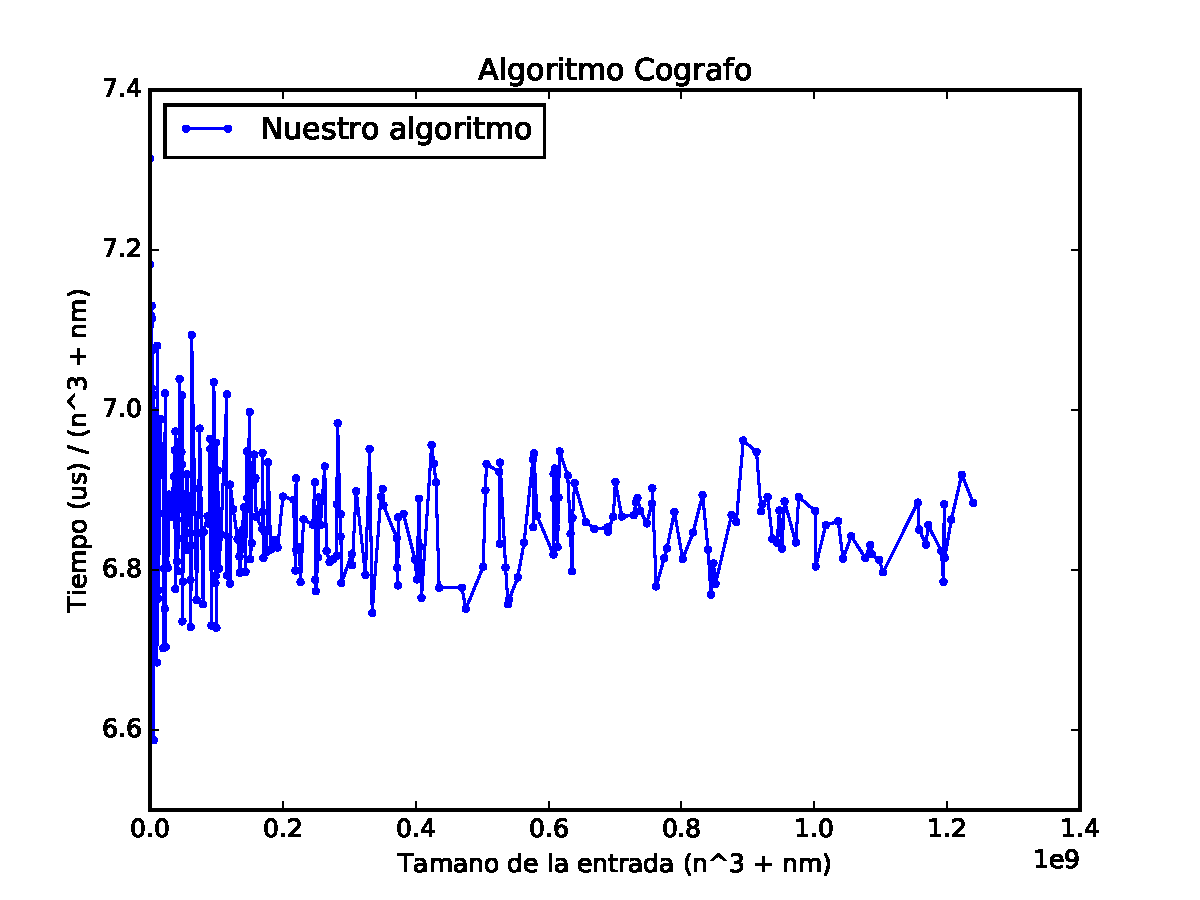
\includegraphics[width=0.8\textwidth]{graficos/problema_3/tiempos0.pdf}
	\caption{}
	\label{fig:problema3-tiempos0}
\end{figure}

Con este experimento confirmamos lo que esperabamos, dado que se ve que el cociente entre tiempo y tamaño de entrada está acotado por una constante, que es lo que queremos que pase, como dijimos en la introducción.

Además, podemos comprobar que si fijamos $n$, todo anda como debería, es decir, la complejidad es lineal en $m$.

\begin{figure}[H]
 \centering
	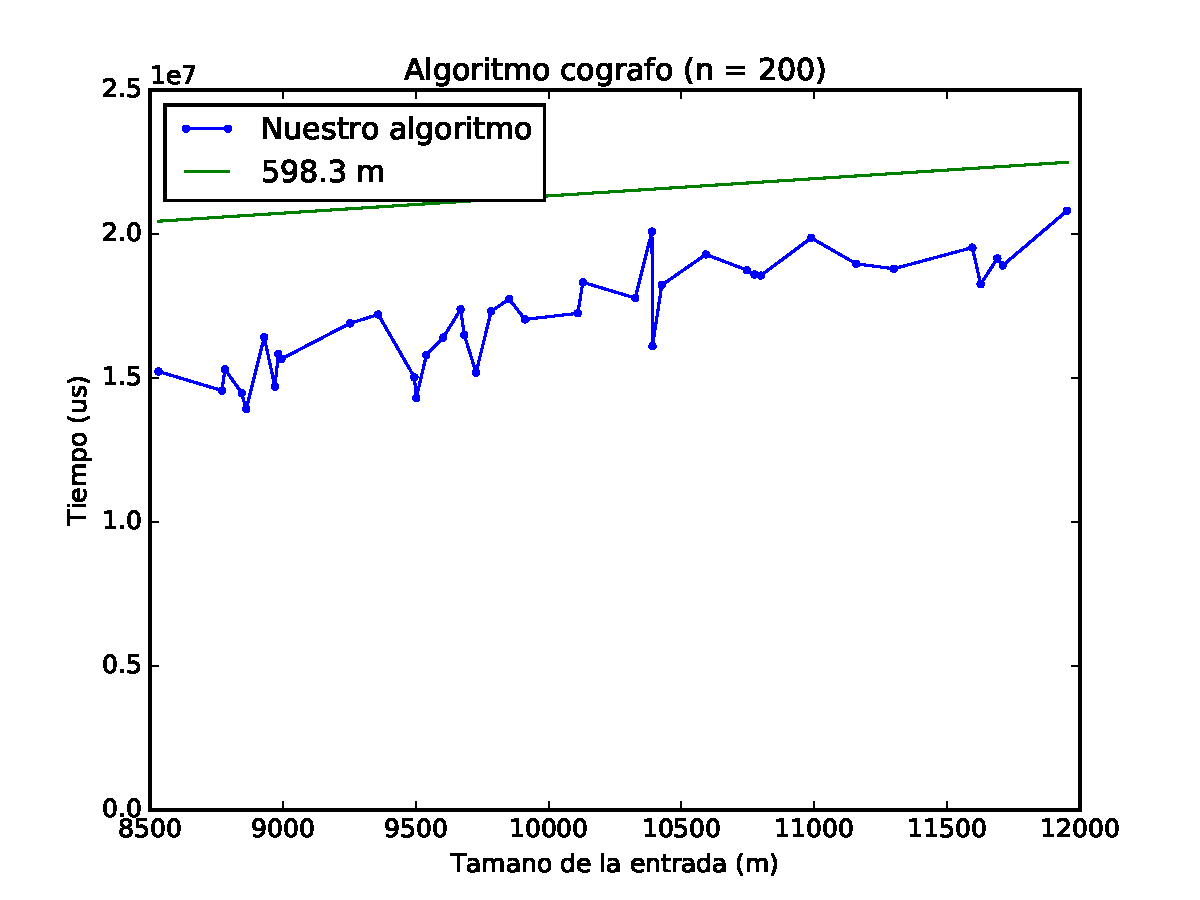
\includegraphics[width=0.8\textwidth]{graficos/problema_3/tiempos1.pdf}
	\caption{}
	\label{fig:problema3-tiempos1}
\end{figure}

Por último, por completitud, es importante decir que es muy díficil, de hecho imposible, hacer el experimento en el que se fija $m$ y se varia $n$, porque nada nos garantiza  que existan suficientes cografos con cantidad de aristas $m$ de distinto $n$ como para hacer un experimento significativo, y además no es claro como generarlos (es decir, dado un $m$ como encontrar todos o varios cografos de distintos $n$).


\subsection{Generación y testing de casos random}

Para testear la correctitud del algoritmo, primero se ejecutó el mismo con grafos de entrada más chicos y se comparó la solución con el algoritmo exacto (Problema anterior). Además, se implementó un generador de cografos random para calcular la performance, testear la correctitud y utilizar como parámetro de comparación en la posterior experimentación de las heurísticas.
A continuación se presenta un algoritmo para generar cografos de manera random:

\begin{algorithm}[H]
  \begin{algorithmic}[1]
  \caption{Pseudocódigo del constructor random de un CographTree}
  \label{algo:3-3}
  \Procedure{CographTree}{\texttt{int} $size$, \texttt{int} $nodoInicial$}
	\State \Comment $nodoInicial$ corresponde al id del primer nodo.
	\State $n = size$
	\For { $i \in [nodoInicial .. nodoInicial + size]$ }
		\State $nodos.agregar(i)$ 
	\EndFor
	\State $sol = <false, Solucion>(n+1)$
	\If { $size == 1$ }
		\State $tipo = trivial$
		\State $izq = null$
		\State $der = null$
	\Else
		\State $nodosIzq = (rand()$ \texttt{mod} $(n-1)) + 1 $
		\State $nodosDer = n - nodosIzq$
		\State $izq = CographTree(nodosIzq, nodoInicial)$
		\State $der = CographTree(nodosDer, nodoInicial + nodosIzq)$
		\State \texttt{int} $trand = rand()$ \texttt{mod} $2$
		\If { $trand == 0$ }
			\State $tipo = unionDisjunta$
			\State $m = izq.m + der.m$
		\Else
			\State $tipo = join$
			\State $m = izq.m + der.m + (nodosIzq * nodosDer)$
		\EndIf
	\EndIf		
  \EndProcedure
  \end{algorithmic}
\end{algorithm}

Junto con el informe y el resto de los problemas se agrega un archivo \texttt{testerproblema3}, que puede ser utilizado para generar casos random y chequear correctitud de los mismos usando el algoritmo planteado anteriormente.

%\subsection{Comparación de las heurísticas para el problema aplicado a cografos}

